\documentclass[a4paper, table]{article}
% Useful packages, sorted so packages of similar functionality are grouped together. Not all are essential to make the document work, however an effort was made to make this list as minimalistic as possible. Feel free to add your own!

% Essential for making this template work are graphicx, float, tabularx, tabu, tocbibind, titlesec, fancyhdr, xcolor and tikz. 

% Not essential, but you will have to debug the document a little bit when removing them are amsmath, amsthm, amssymb, amsfonts, caption, subcaption, appendix, enumitem, hyperref and cleveref.

% inputenc, lipsum, booktabs, geometry and microtype are not required, but nice to have.

\usepackage[utf8]{inputenc} % Allows the use of some special characters
\usepackage{amsmath, amsthm, amssymb, amsfonts} % Nicer mathematical typesetting
\usepackage{lipsum} % Creates dummy text lorem ipsum to showcase typsetting 

\usepackage{graphicx} % Allows the use of \begin{figure} and \includegraphics
\usepackage{float} % Useful for specifying the location of a figure ([H] for ex.)
\usepackage{caption} % Adds additional customization for (figure) captions
\usepackage{subcaption} % Needed to create sub-figures

\usepackage{tabularx} % Adds additional customization for tables
\usepackage{tabu} % Adds additional customization for tables
\usepackage{makecell} % Adds additional customization for cells
\usepackage{booktabs} % For generally nicer looking tables

\usepackage[nottoc,numbib]{tocbibind} % Automatically adds bibliography to ToC
\usepackage[margin = 2.5cm]{geometry} % Allows for custom (wider) margins
\usepackage{microtype} % Slightly loosens margin restrictions for nicer spacing  
\usepackage{titlesec} % Used to create custom section and subsection titles
\usepackage{titletoc} % Used to create a custom ToC
\usepackage{appendix} % Any chapter after \appendix is given a letter as index
\usepackage{fancyhdr} % Adds customization for headers and footers
\usepackage[shortlabels]{enumitem} % Adds additional customization for itemize. 

\usepackage{hyperref} % Allows links and makes references and the ToC clickable
\usepackage[noabbrev, capitalise]{cleveref} % Easier referencing using \cref{<label>} instead of \ref{}

\usepackage{xcolor} % Predefines additional colors and allows user defined colors

\usepackage{tikz} % Useful for drawing images, used for creating the frontpage
\usetikzlibrary{positioning} % Additional library for relative positioning 
\usetikzlibrary{calc} % Additional library for calculating within tikz

\usepackage{listings}

% Defines a command used by tikz to calculate some coordinates for the front-page
\makeatletter
\newcommand{\gettikzxy}[3]{%
  \tikz@scan@one@point\pgfutil@firstofone#1\relax
  \edef#2{\the\pgf@x}%
  \edef#3{\the\pgf@y}%
}
\makeatother

\definecolor{dkgreen}{rgb}{0,0.6,0}
\definecolor{gray}{rgb}{0.5,0.5,0.5}
\definecolor{mauve}{rgb}{0.58,0,0.82}

\lstset{frame=tb,
  language=Java,
  aboveskip=3mm,
  belowskip=3mm,
  showstringspaces=false,
  columns=flexible,
  basicstyle={\small\ttfamily},
  numbers=none,
  numberstyle=\tiny\color{gray},
  keywordstyle=\color{blue},
  commentstyle=\color{dkgreen},
  stringstyle=\color{mauve},
  breaklines=true,
  breakatwhitespace=true,
  tabsize=3
}

 % Loads in the preamble 
% Give your report a title
\newcommand\reporttitle{Project}

% Insert course code, name, quartile number and year (or any other subtitle)
\newcommand\reportsubtitle{
BCS1110, Introduction to Computer Science
}

% Add your group number (for DBL) or any other text.
\newcommand\groupnumber{
\textbf{Group 11}
}

% Insert authors and student numbers here
\newcommand\reportauthors{
Long Luong & I6359380\\
Élisa Donéa & I6356213\\
Chris Munteanu & I6344912\\
Alexia Raportaru & I6355814\\
}

% Add the name of your tutor (for DBL) or any other text.
\newcommand\grouptutor{
Professors: Dr. Ashish Sai, Dr. Thomas Bitterman
}

% Date and location (default: current date and Eindhoven)
\newcommand\placeanddate{
Maastricht, \today
}

% Define Tue-red (color of the TU/e logo). Can be changed to drastically change the look of the template
\definecolor{Tue-red}{RGB}{0, 25, 58}

% All of the following code can be removed to be left with (close to) default LaTeX behaviour. 

% Sets up hyperlinks in the document to be colored
\hypersetup{
    colorlinks=true,
    linkcolor=Tue-red,
    urlcolor=Tue-red,
    citecolor = Tue-red
    }
\urlstyle{same} % Defines settings for link and reference formatting


% Change bullet style for level 1, 2 and 3 respectively for itemize
\renewcommand{\labelitemi}{\scriptsize\textcolor{Tue-red}{$\blacksquare$}}% level 1
\renewcommand{\labelitemii}{\scriptsize\textcolor{Tue-red}{$\square$}}% level 2
\renewcommand{\labelitemiii}{\textcolor{Tue-red}{$\circ$}}% level 3

% \renewcommand{\labelitemi}{\small\textcolor{Tue-red}{\ding{70}}} % level 1
% \renewcommand{\labelitemii}{\small\textcolor{Tue-red}{\ding{71}}}% level 2
% \renewcommand{\labelitemiii}{\tiny\textcolor{Tue-red}{\ding{71}}}% level 3

% Change bullet style for level 1, 2 and 3 respectively for enumerate
\renewcommand{\labelenumi}{\textbf{\textcolor{Tue-red}{\arabic*.}}}% level 1
\renewcommand{\labelenumii}{\textbf{\textcolor{Tue-red}{[\alph*]}}}% level 2
\renewcommand{\labelenumiii}{\textbf{\textcolor{Tue-red}{\roman*.}}}% level 3

% Have reference labels be linked to section (section 3 will have fig. 3.1 etc.)
\counterwithin{equation}{section} % For equations
\counterwithin{figure}{section} % For figures
\counterwithin{table}{section} % For tables

% Creates a beautiful header/footer
\pagestyle{fancy}
\lhead{
\includegraphics[height = 16pt]{Figures/0. General/maastricht-logo-wide.png}}
\rhead{\reporttitle}
\renewcommand{\footrulewidth}{0.4pt}
\cfoot{Page \thepage}

% Formats section, subsection and subsubsection titles respectively 
\titleformat{\section}{\sffamily\color{Tue-red}\Large\bfseries}{\thesection\enskip\color{gray}\textbar\enskip}{0cm}{} % Formats section titles

\titleformat{\subsection}{\sffamily\color{Tue-red}\large\bfseries}{\thesubsection\enskip\color{gray}\textbar\enskip}{0cm}{} % Formats subsection titles

\titleformat{\subsubsection}{\sffamily\color{Tue-red}\bfseries}{\thesubsubsection\enskip\color{gray}\textbar\enskip}{0cm}{} % Formats subsubsection titles

% Formats captions
\DeclareCaptionFont{Tue-red}{\color{Tue-red}}
\captionsetup{labelfont={Tue-red,bf}}

 % Changes font to mlmodern
\usepackage{mlmodern}

% Removes indent when starting a new paragraph
\setlength\parindent{0pt}

% Limits the ToC to sections and subsections (no subsubsec.)
\setcounter{tocdepth}{2}
 % Loads in user defined settings
\begin{document}

% Inserts the front page
\begin{titlepage}

\centering

{
\includegraphics[width=.4\textwidth]{Figures/0. General/maastricht-logo.png}}

\vspace{1cm}
    
{\sffamily\huge\reporttitle}

\vspace{0.5cm}

{\sffamily\Large \reportsubtitle}

\vspace{2cm}

\sffamily\groupnumber

\begin{table}[H]
\centering
\sffamily
\large
\begin{tabu} to 0.8\linewidth {cc}
\textbf{Full Name} & \textbf{Student ID}\\
\hline

\sffamily\reportauthors

\end{tabu}

\end{table}

\sffamily \grouptutor

% \tikz[remember picture,overlay]\node[anchor=south,inner sep=0pt] at (current page.south) {
\includegraphics[width=\paperwidth]{Figures/0. General/city.jpg}};

\mbox{}
\vfill
\sffamily \Large \textcolor{black}{\placeanddate} \\



\end{titlepage}









\newpage

% Generates a ToC without page number
{\hypersetup{linkcolor=black} % Keeps the ToC black even with non-black linkcolor
\tableofcontents\thispagestyle{empty}}
\newpage

% contains inspiration for formatting tables, images, text citations etc.
% \section{Introduction} \pagenumbering{roman}
\subsection{This is a subsection}

\subsubsection{This is a subsubsection}
This section contains some templates that can be used to create a uniform style within the document. It also shows of the overall formatting of the template, created using the predefined styles from the \texttt{settings.tex} file.

\subsection{General formatting}
Firstly, the document uses the font mlmodern, using no indent for new paragraphs and commonly uses the color \textcolor{Tue-red}{Tue-red} (the color of the TU/e logo) in its formatting. It uses the \texttt{fancyhdr} package for its headers and footers, using the TU/e logo and report title as the header and the page number as the footer. The template uses custom section, subsection and subsubsection formatting making use of the \texttt{titlesec} package.\\
The \texttt{hyperref} package is responsible for highlighting and formatting references like figures and tables. For example \cref{table: style 1} or \cref{fig: three images}. It also works for citations \cite{texbook}. Note how figure numbers are numbered according to the format \texttt{<chapter number>.<figure number>}.\\

Bullet lists are also changed globally, for a maximum of 3 levels:

\begin{itemize}
    \item Item 1
    \item Item 2
    \begin{itemize}
        \item subitem 1
        \begin{itemize}
            \item subsubitem 1
            \item subsubitem 2
        \end{itemize}
    \end{itemize}
    \item Item 3
\end{itemize}

Similarly numbered lists are also changed document wide:

\begin{enumerate}
    \item Item 1
    \item Item 2
    \begin{enumerate}
        \item subitem 1
        \begin{enumerate}
            \item subsubitem 1
            \item subsubitem 2
        \end{enumerate}
    \end{enumerate}
    \item Item 3
\end{enumerate}

\newpage

\subsection{Tables and figures}
The following table, \cref{table: style 1}, shows a possible format for tables in this document. Alternatively, one can also use the black and white version of this, shown in \cref{table: style 2}. Note that caption labels are in the format \textbf{\textcolor{Tue-red}{Table x.y:} }
\begin{table}[ht]
\rowcolors{2}{Tue-red!10}{white}
\centering
\caption{A table without vertical lines.}
\begin{tabular}[t]{ccccc}
\toprule
\color{Tue-red}\textbf{Column 1}&\color{Tue-red}\textbf{Column 2}&\color{Tue-red}\textbf{Column 3}&\color{Tue-red}\textbf{Column 4}&\color{Tue-red}\textbf{Column 5}\\
\midrule
Entry 1&1&2&3&4\\
Entry 2&1&2&3&4\\
Entry 3&1&2&3&4\\
Entry 4&1&2&3&4\\
\bottomrule
\end{tabular}
\label{table: style 1}
\end{table}

\begin{table}[ht]
\rowcolors{2}{gray!10}{white}
\centering
\caption{A table without vertical lines.}
\begin{tabular}[t]{ccccc}
\toprule
\textbf{Column 1}&\textbf{Column 2}&\textbf{Column 3}&\textbf{Column 4}&\textbf{Column 5}\\
\midrule
Entry 1&1&2&3&4\\
Entry 2&1&2&3&4\\
Entry 3&1&2&3&4\\
Entry 4&1&2&3&4\\
\bottomrule
\end{tabular}
\label{table: style 2}
\end{table}

For normal, single image figures, the standard \texttt{\textbackslash begin\{figure\}} environment can be used. For multi-image figures, one could use either the \texttt{\textbackslash begin\{subfigure\}} environment to get a main caption with 3 subcaptions like \cref{fig: three images} or the \texttt{\textbackslash begin\{minipage\}} environment to get 3 independent captions like \cref{fig: style 2 image a} - \ref{fig: style 2 image c}

\begin{figure}[H]
     \centering
     \begin{subfigure}[b]{0.3\textwidth}
         \centering
         \includegraphics[width=\textwidth]{example-image-a}
         \caption{image a}
         \label{fig: style 1 image a}
     \end{subfigure}
     \hfill
     \begin{subfigure}[b]{0.3\textwidth}
         \centering
         \includegraphics[width=\textwidth]{example-image-b}
         \caption{image b}
         \label{fig: style 1 image b}
     \end{subfigure}
     \hfill
     \begin{subfigure}[b]{0.3\textwidth}
         \centering
         \includegraphics[width=\textwidth]{example-image-c}
         \caption{image c}
         \label{fig: style 1 image c}
     \end{subfigure}
        \caption{Three images}
        \label{fig: three images}
\end{figure}

\begin{figure}[H]
\centering
\begin{minipage}{0.3\textwidth}
  \centering
  \includegraphics[width=\textwidth]{example-image-a}
  \captionof{figure}{image a}
  \label{fig: style 2 image a}
\end{minipage}
\hfill
\begin{minipage}{0.3\textwidth}
  \centering
  \includegraphics[width=\textwidth]{example-image-b}
  \captionof{figure}{image b}
  \label{fig: style 2 image b}
\end{minipage}
\hfill
\begin{minipage}{0.3\textwidth}
  \centering
  \includegraphics[width=\textwidth]{example-image-c}
  \captionof{figure}{image c}
  \label{fig: style 2 image c}
\end{minipage}
\end{figure} % Feel free to remove / comment out
% \newpage

% Creates the introduction, starting page numbering
\section{Introduction} \label{section: introduction}
JavaCraft is a a multifaceted text-based Java game inspired by Minecraft. The game is a relatively complex Java program that brings over 35 functions to create a diverse gameplay experience. This team project is an academic exercise in computer science, logical thinking, and collaboration. Working in teams of four, we used our creativity, analytical skills, and technical skills to analyse and expand upon the existing JavaCraft game. The source code of JavaCraft can be found in the following link: \url{https://gitlab.maastrichtuniversity.nl/bcs1110/javacraft/-/raw/main/JavaCraft.java} \\

Below is a table that describes what each team member did on the project, divided by section:

\begin{center}
    \begin{tabular}{ l l }
     Section & Who did what\\
     \hline
     Introduction & Long (100\%)\\  
     JavaCraft's Workflow & Alexia (100\%) \\
     Functionality Exploration & Long (60\%), Élisa (40\%) \\
     Secret Door FSA Design & Élisa (50\%), Chris (50\%) \\
     Git Collaboration \& Version Control & Alexia (25\%), Élisa (25\%), Chris (25\%), Long (25\%) \\
     Pseudocode \& flowcharts for 15 different functions & Alexia (31\%), Élisa (31\%), Chris (31\%), Long (7\%) \\
     Report & Long (100\%) \\ 
    \end{tabular}
\end{center}
 \pagenumbering{arabic}
\newpage

\section{JavaCraft's Workflow} \label{section: javacraft workflow}
In order to fully understand the mechanism of the game, a flowchart of the entire game is provided below. The flowchart is accompanied by pseudocode.

{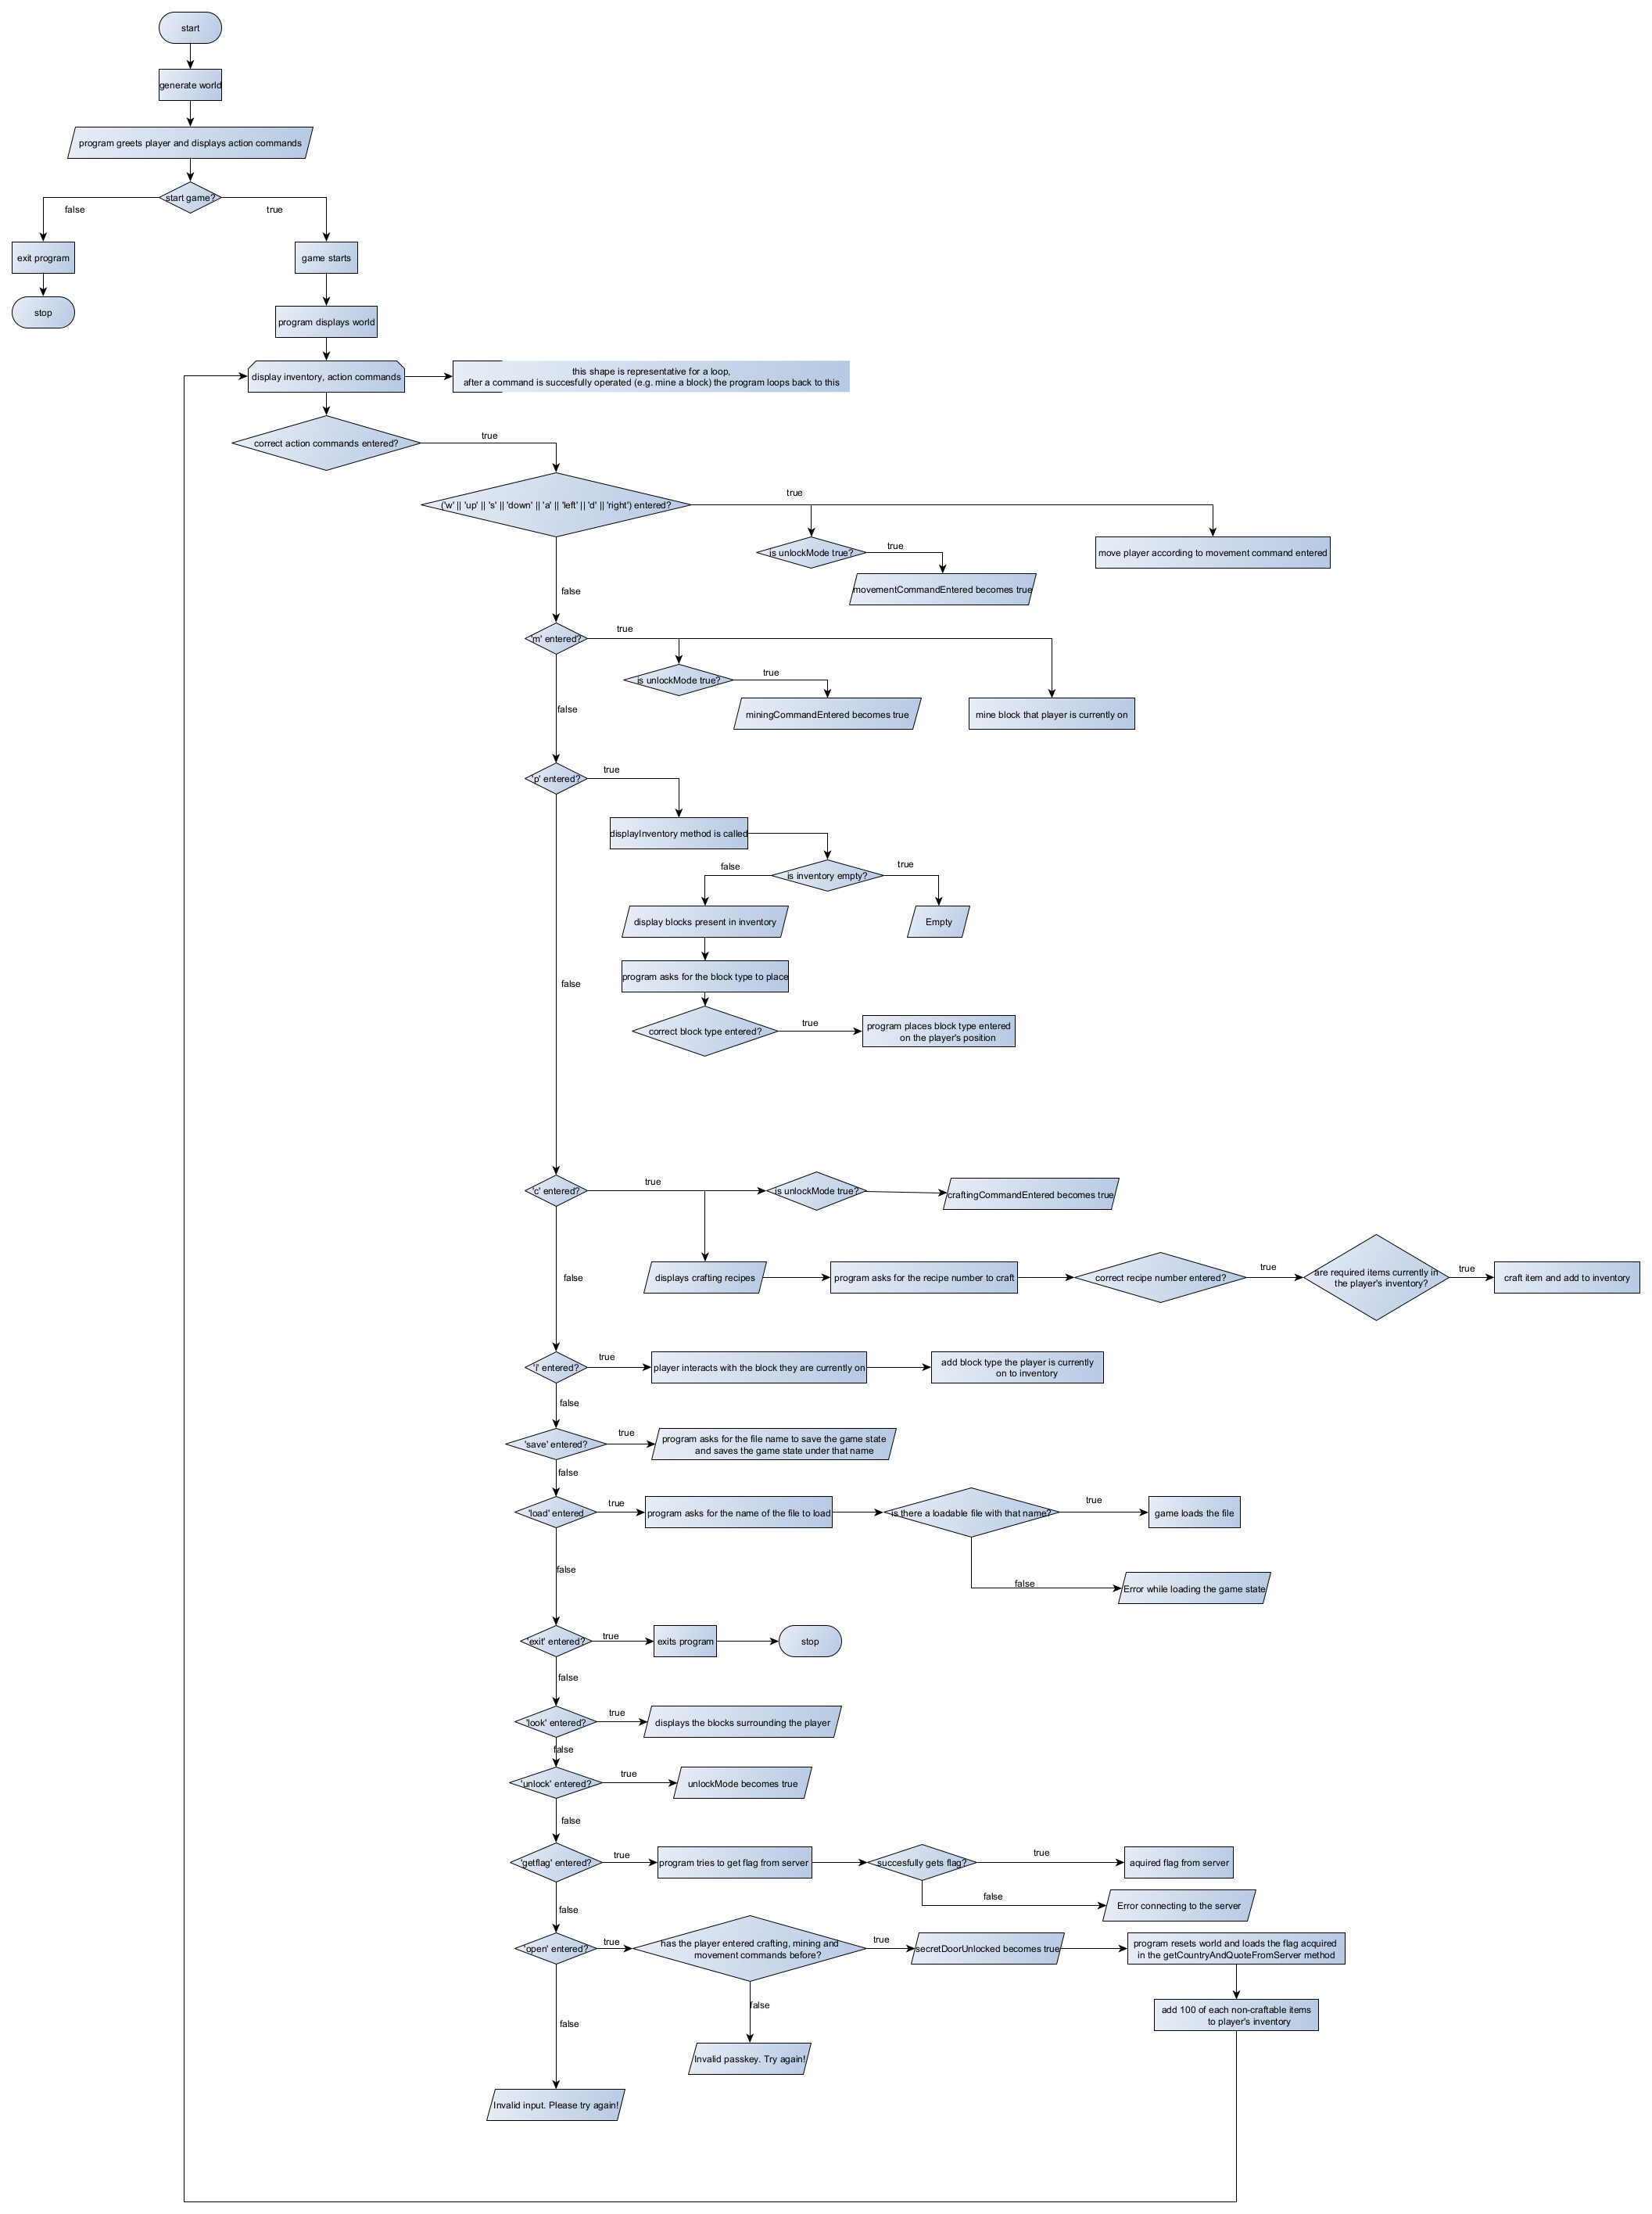
\includegraphics[width=\textwidth,height=\textheight,keepaspectratio]{../flowchart/WorkFlow_of_JavaCraft.png}}

\begin{lstlisting}
    generate world
    print welcome message and instructions
    ask player if they want to start the game
    if choice is equal to 'y' then start game 
       clear screen
       display world
    
       loop
       display inventory, display legend
    
       if input is 'wasd' then move player accordingly 
          if unlockMode is true then movementCommandEntered becomes true
    
       else if input is 'm' then mine the block the player is currently standing on
          if unlockMode is true then miningCommandEntered becomes true
    
       else if input is 'p' then function displayInventory and ask player which block they want to place                                               	if inventory is empty display "Empty"
        else display inventory
          if input is correct then place block on the player's current position
          else inform player they do not have that specific block in their inventory
    
       else if input is 'c' then display crafting recipes 
          ask for recipe number in order to craft 
              if input is correct then check whether the player has the items necessary for the crafting recipe
                  if the player has the necessary items then proceed crafting and add the item to the player's inventory
                  else inform the player they have insufficient resources to craft
          if unlockMode is true then craftinCommandEntered becomes true
       
       else if input is 'i' then player interacts with the block they are currently standing on
          if the block they are currently on is not air then add the item to their inventory
    
       else if input is 'save' then ask player for a name for the current state file they want to save
          save file
    
       else if input is 'load' then ask player for the name of the file they want to load
          if there is a file with that name then load file
          else inform player there has been an error loading the game state
    
       else if input is 'exit' then exit program
    
       else if input is 'look' then inform the player of the block types surrounding them
    
       else if input is 'unlock' then unlockMode becomes true
       
       else if input is 'getflag' then try to get flag from the server
          if unsuccesful then inform the player that there has been an error connecting to the server
    
       else if input is 'open' then check if the booleans craftingCommandEntered, movementCommandEntered, miningCommandEntered true
          if they are true then secretDoorUnlocked becomes true 
             reset world
             load flag world
             add 100 of leaves, stone, iron ore and wood to player's inventory
    
       else inform player that their input is invalid
    end if
    else print "Game not started. Goodbye!" and exit program
    end if
\end{lstlisting}

\newpage

\section{Functionality Exploration} \label{section: functionality exploration}

\begin{table}[ht]
    \rowcolors{2}{gray!10}{white}
    \centering
    \caption{A table that describes functions used in javacraft}
    \begin{tabular}[t]{ccccc}
    \toprule
    \textbf{No.}&\textbf{Function Name}&\textbf{Description}\\
    \midrule
    Entry 1& \texttt{void generateWorld} & assigns integer to every tile of the world\\
    Entry 2& \texttt{void initGame} & creates world with width \texttt{worldWidth} and height \texttt{worldHeight}\\
    Entry 3& \texttt{void main} & main function\\
    Entry 4& \texttt{void startGame} & starts the game\\
    Entry 5& \texttt{void movePlayer} & moves player horizontally or vertically\\
    Entry 6& \texttt{void mineBlock} & mines block player is on if block is not air\\
    Entry 7& \texttt{String getBlockSymbol} & returns symbol of \texttt{blockType}\\
    Entry 8& \texttt{void resetWorld} & clears the world and sets player position in middle\\
    Entry 9& \texttt{void generateEmptyWorld} & generates an empty world\\
    Entry 10& \texttt{void clearScreen} & clears terminal\\
    Entry 11& \texttt{void lookAround} & prints out adjacent squares to player\\
    Entry 12& \texttt{void fillInventory} & completely fills up inventory of player\\
    Entry 13& \texttt{void displayLegend} & displays a legend of what each tile represents\\
    Entry 14& \texttt{void displayWorld} & prints out all tiles of the world\\
    Entry 15& \texttt{void displayInventory} & prints out obtained items \& crafted items\\
    Entry 16& \texttt{void loadGame} & loads the game from file \texttt{fileName}\\
    Entry 17& \texttt{void saveGame} & saves the game in file \texttt{fileName}\\
    Entry 18& \texttt{void interactWithWorld} & interacts with item player is standing on\\
    Entry 19& \texttt{void addCraftedItem} & adds item \texttt{craftedItem} to array \texttt{craftedItems} \\
    Entry 20& \texttt{void removeItemsFromInventory} & removes item \texttt{item} \texttt{count} times from inventory\\
    Entry 21& \texttt{boolean inventoryContains} & returns boolean of whether \texttt{item} is in inventory\\
    Entry 22& \texttt{void placeBlock} & places block \texttt{blockType} at player position\\
    Entry 23& \texttt{void displayCraftingRecipes} & prints out available crafting recipes\\
    Entry 24& \texttt{void craftItem} & crafts an item based on argument \texttt{recipe}\\
    Entry 25& \texttt{void craftIronIngot} & crafts an iron ingot\\
    Entry 26& \texttt{void craftStick} & crafts a stick\\
    Entry 27& \texttt{void waitForEnter} & waits for operator to press Enter\\
    Entry 28& \texttt{String getBlockTypeFromCraftedItem} & returns integer of \texttt{craftedItem}\\
    Entry 29& \texttt{String getCraftedItemFromBlockType} & returns integer of \texttt{blockType}\\
    Entry 30& \texttt{String getBlockName} & returns name of \texttt{blockType}\\
    Entry 31& \texttt{String getBlockColor} & returns color of \texttt{blockType}\\
    Entry 32& \texttt{String getCraftedItemName} & returns name of \texttt{craftedItem}\\
    Entry 33& \texttt{String getCraftedItemColor} & returns color of \texttt{craftedItem}\\
    Entry 34& \texttt{char getBlockChar} & returns char of \texttt{blockType}\\
    Entry 35& \texttt{void craftWoodenPlanks} & crafts wooden planks\\
    Entry 36& \texttt{void getCountryAndQuoteFromServer} & fetches HTTP request from and writes data to server and prints country and quote\\
    \bottomrule
    \end{tabular}
    \label{table: style 2}
\end{table}
\newpage

\section{Finite State Automata (FSA) Design} \label{section: fsa design}
The following describes the Secret Door Logic through an FSA illustration and a description: \\
{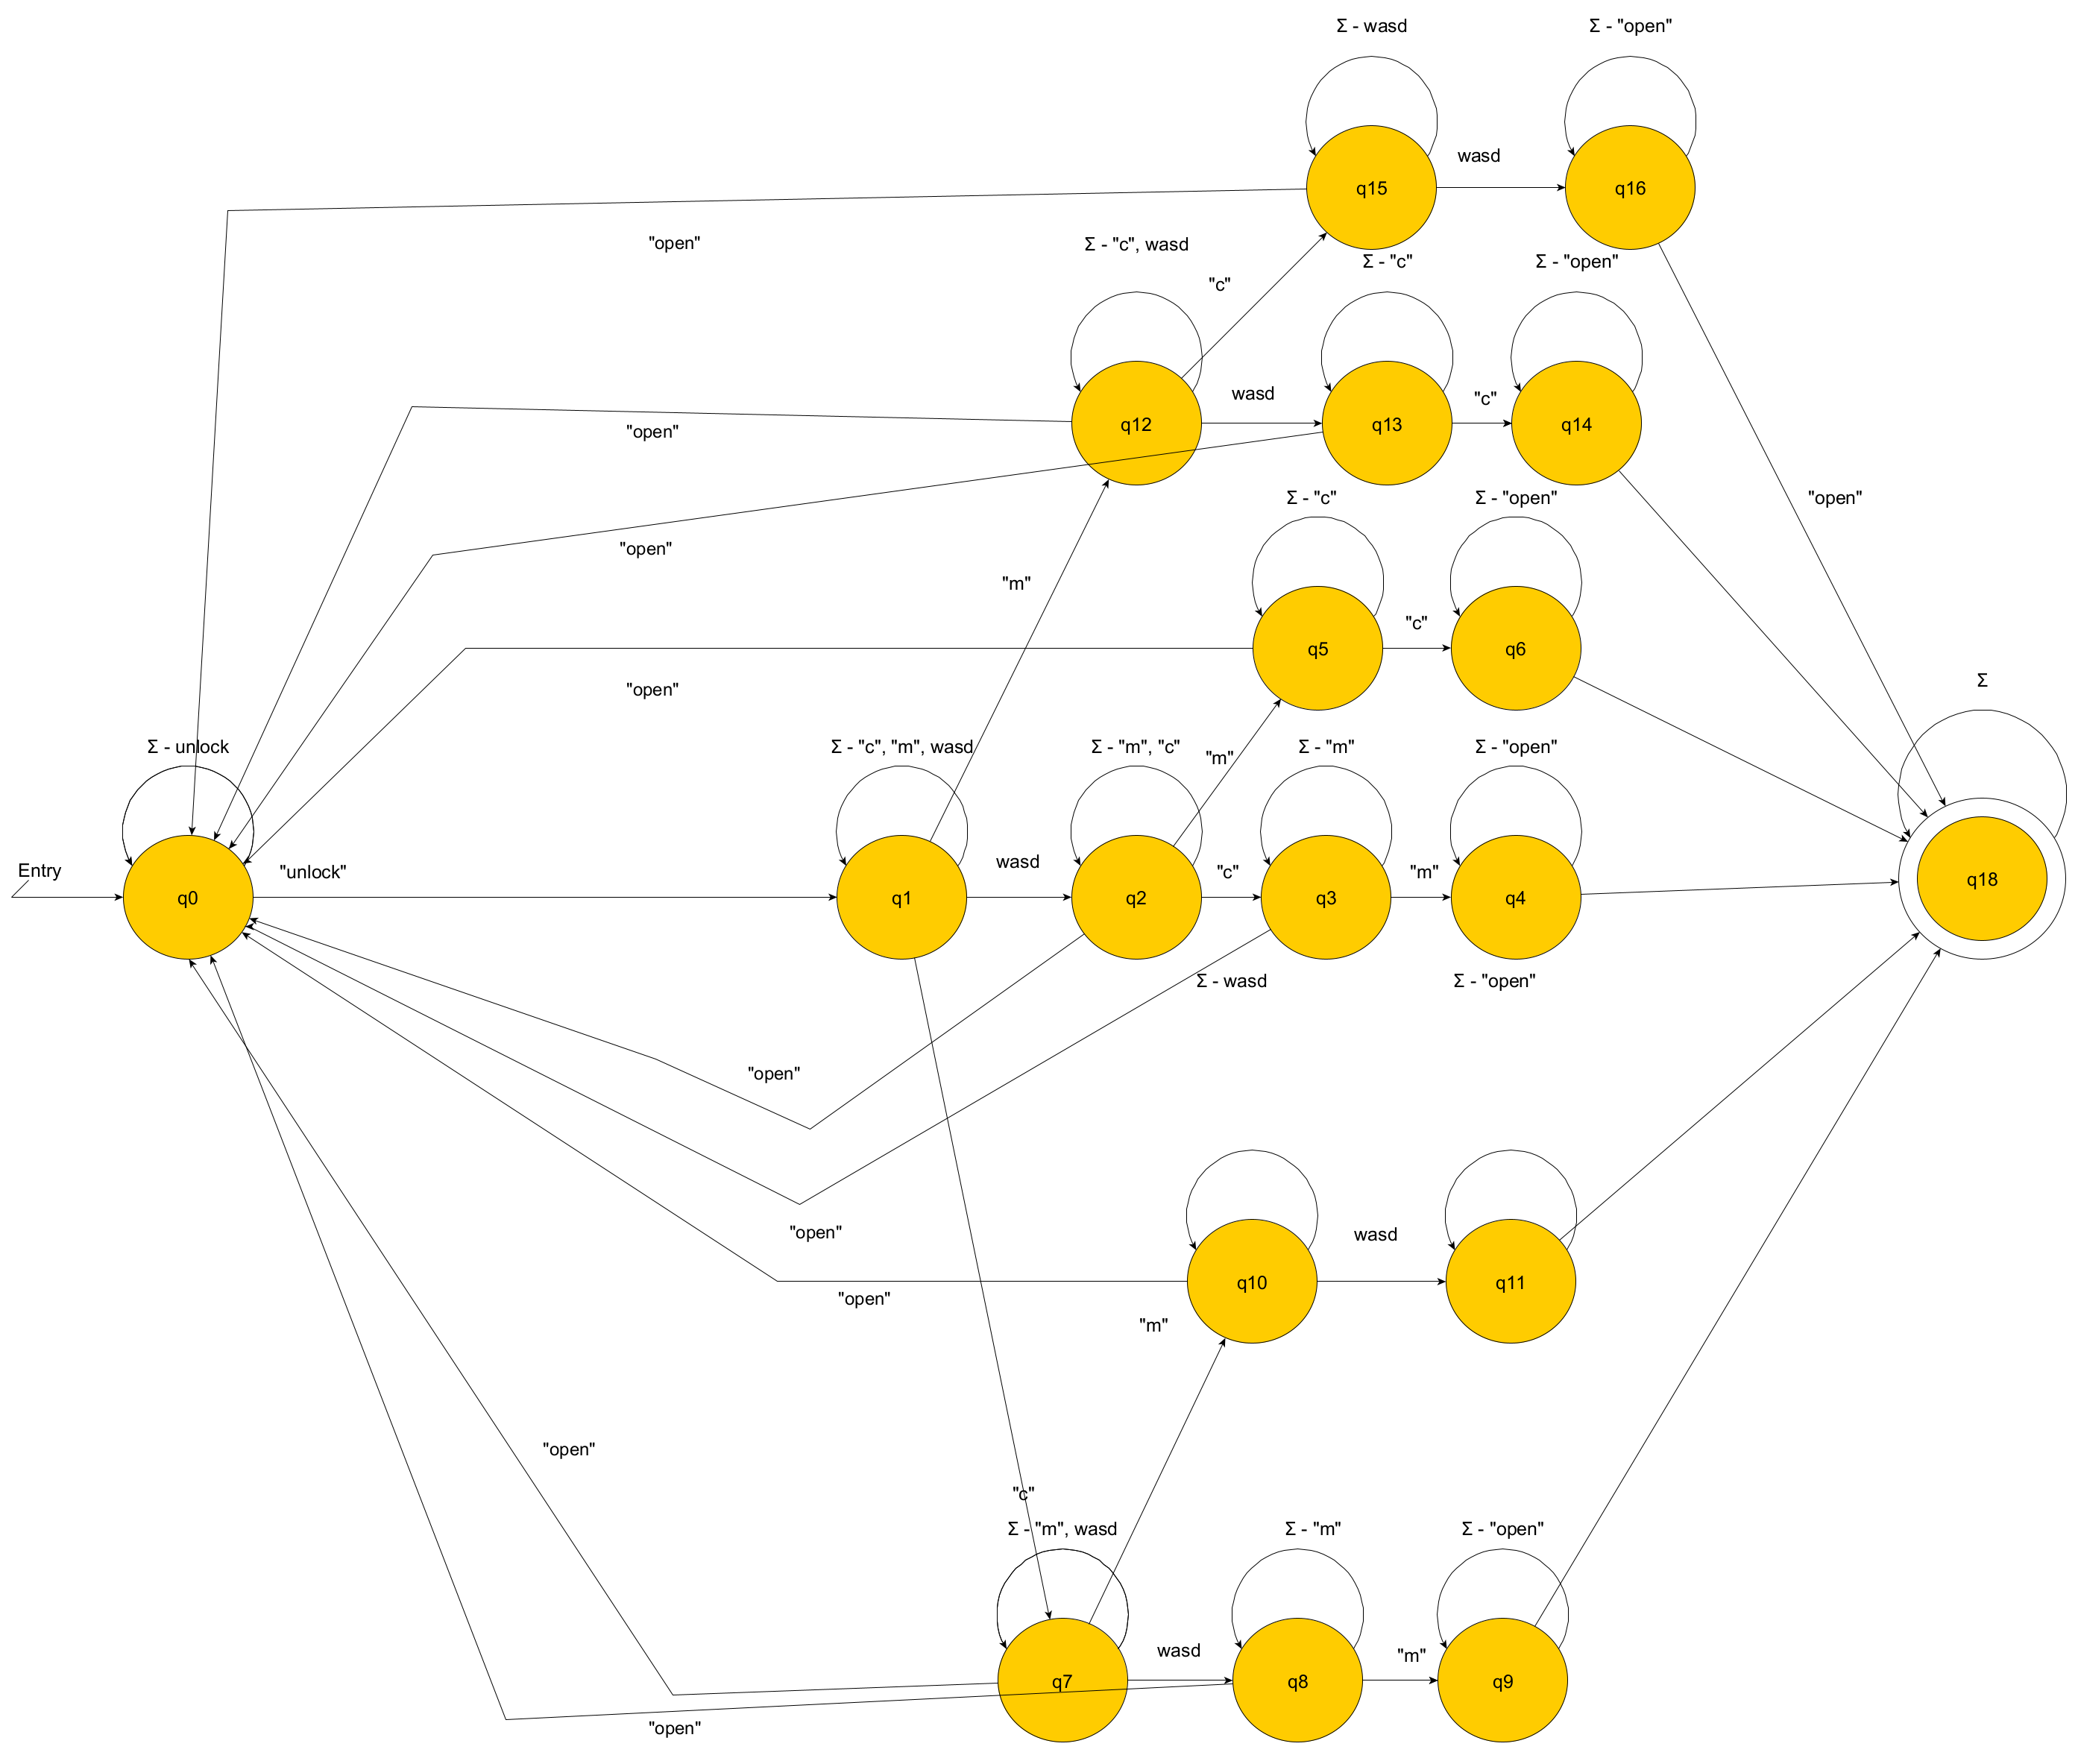
\includegraphics[width=\textwidth,height=\textheight,keepaspectratio]{../dfa.png}}

We have 18 finite set of states and in our alphabet we have "open" , "wasd", "c", "m" and "unlock" 
On step one Q0 you have to write unlock if not you will remain in Q0
After you have arrived  in Q1 you have the choice in between wasd, c, m because in able to unlock the secret door you must c, craft then m, mine or wasd to move in any order that's why after Q1 it divides in 3 because the order is not important.
If you type a move command (w,a,s or d) you enter Q2, the only options you have from now are mine or craft if not you stay in Q2 unless you type open which sends you back to Q0 and have to start again. If you type c you go into Q3 so the last thing you have to write is mine if you write anything else you stay in Q3 expect "open" which sends you in Q0 after mining you enter Q4. From there your only option is to "open" which unlocks the secret door.
Now because the order doesn't matter after Q2  you can also type m for mine which sends you in Q5 where the only option is c, "craft" if you type anything else you go back to Q0 after you type C you entre Q6 where you can only type "open" which will unlock the secret door.
We have created 2 other branches based on the same principal so we can cover all the possible ways you can acces the secret door

Note: in our alphabet "wasd" stands for "w", "a", "s" or "d" 

\newpage

\section{Git Collaboration \& Version Control} \label{section: git}
The link to the JavaCraft branch can be found here: \href{https://gitlab.maastrichtuniversity.nl/bcs1110/javacraft/-/tree/group11}{https://gitlab.maastrichtuniversity.nl/bcs1110/javacraft/-/tree/group11} \\

All the files of the project can be found in the repository. \\ 
Everything was done on one branch called group11. There were no conflicts during the process.
\newpage

% \section{Team Overview} \label{section: overview}
Below describes what each team member did on the project:

\subsection{Long Luong} 
Project leader \\
LaTeX Document owner and composer \\
Created 1 flowchart with pseudocode: \\
1. getCountryAndQuoteFromServer \\
Finalised the Function Exploration part \\
Helped others with git issues \\
Refined some pseudocode that others have made

\subsection{Élisa Donéa}

Designed FSA for secret door with Chris \\
Initiated with the Function Exploration \\
Create 5 flowcharts with pseudocode: \\
1. fillInventory \\
2. generateEmptyWorld \\
3. generateWorld \\
4. initGame \\
5. lookAround \\

\subsection{Chris Munteanu}

Designed FSA for secret door with Élisa \\
Create 5 flowcharts with pseudocode: \\
1. displayInventory \\
2. getBlockName \\
3. loadGame \\
4. removeItemsFromInventory \\
5. saveGame \\

\subsection{Alexia Raportaru}

Create 5 flowcharts with pseudocode: \\
1. placeBlock \\
2. craftItem \\
3. interactWithWorld \\
4. mineBlock \\
5. movePlayer \\
Created an impressive flowchart of the entire game along with its pseudocode explanation

\subsection{Explanation}

When we first met up with each other we were with the three of us. During the first week we got to know each other. Long proposed to be the document manager because he knows how to use LaTeX. He also created a (now deprecated) GitLab repository found at [URL]. During the second week Alexia joined the group. We met up with each other and we divided the roles. We had to create at least 16 flowcharts alongside with pseudocode. Long mentioned that most of the functions are vey easy to understand, and since he wanted a difficult one he proposed to do the function getCountryAndQuoteFromServer and he proposed the other three group members to do 5 flowcharts with their respective pseudocode. Everybody agreed and thinks it is a good idea.
In week 3 Élisa and Chris decided to work on the FSA together. Everybody in the group was new to Git except Long, so he helped out everyone set-up the Git environment and he explained to everyone how it works.  In the meantime, Alexia worked on the flowchart and the pseudocode of the entire game JavaCraft. Later, Long found out he made a mistake and that we had to create a branch on the repository [LINK] so he informed everybody about the mistake and that we all had to migrate to the correct branch.
% \newpage

% Creates references using the Biblatex 
\bibliographystyle{plain}
\bibliography{General/References.bib}
\newpage

\appendix % Any section after this command will have a letter as an index

% Adds an appendix entry
\section{Appendix: pseudocode and flowcharts} \label{section: appendix}
This appendix provides the full blocks of pseudocode and its flowcharts.

{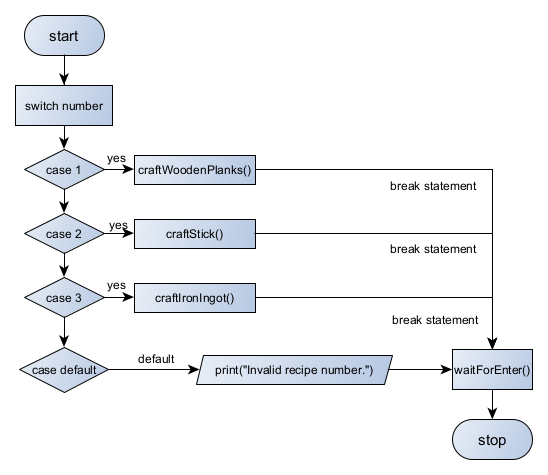
\includegraphics[width=\textwidth]{../flowchart/craftItem_-_Flowchart.png}}
\newpage

\end{document}
